\documentclass[11pt]{article}

\usepackage[a4paper,margin=24mm,headheight=15pt]{geometry}
\usepackage[T1]{fontenc}
\usepackage{lmodern}
\usepackage{microtype}
\usepackage{amsmath,amssymb,mathtools,bm}
\usepackage{booktabs,longtable,tabularx,array,multirow}
\usepackage{graphicx}
\usepackage{caption,subcaption}
\usepackage{float,placeins}
\usepackage[dvipsnames]{xcolor}
\usepackage{tikz}
\usetikzlibrary{arrows.meta,positioning,fit,calc,shapes.geometric}
\usepackage{enumitem}
\usepackage{fancyhdr}
\usepackage{natbib}
\usepackage[hidelinks]{hyperref}
\usepackage[nameinlink,noabbrev]{cleveref}

\definecolor{hsblue}{HTML}{0072B2}
\definecolor{hsgreen}{HTML}{009E73}
\definecolor{hsorange}{HTML}{E69F00}
\definecolor{hspurple}{HTML}{CC79A7}
\definecolor{hsgray}{HTML}{5F6368}
\newcommand{\diffmah}{\textnormal{\textsc{DiffMAH}}}
\newcommand{\cog}{\mathrm{CoG}}
\newcommand{\Msun}{\mathrm{M}_{\odot}}
\newcommand{\Mpeak}{M_{\mathrm{peak}}}
\newcommand{\Rtwo}{R_{200\mathrm{c}}}
\newcommand{\ctwo}{c_{200\mathrm{c}}}
\newcommand{\logten}{\log_{10}}
\newcommand{\given}{\,\middle|\,}
\newcommand{\vect}[1]{\bm{#1}}
\newcommand{\ExpFifty}{Exp50}
\newcommand{\ExpFiftyOne}{Exp51}
\newcommand{\TNG}{\textsc{TNG300}}
\newcommand{\dex}{\,\mathrm{dex}}
\newcommand{\kpc}{\,\mathrm{kpc}}
\newcommand{\gyr}{\,\mathrm{Gyr}}

\captionsetup{font=small,labelfont=bf}
\setlist{itemsep=2pt,topsep=4pt}
\setlength{\parindent}{0pt}
\setlength{\parskip}{5pt plus 1pt}
\renewcommand{\arraystretch}{1.15}
\pagestyle{fancy}
\fancyhf{}
\fancyhead[L]{HongShao: direct halo-to-profile conversion}
\fancyhead[R]{Exp50 and Exp51 working report}
\fancyfoot[C]{\thepage}

\hypersetup{
  pdftitle={A Direct Probabilistic Connection Between Halo Assembly and Massive-Galaxy Curves of Growth},
  pdfauthor={HongShao project},
  pdfsubject={Technical report for experiments 50 and 51},
  pdfkeywords={galaxy-halo connection, DiffMAH, curve of growth, TNG300}
}

\title{\textbf{A Direct Probabilistic Connection Between Halo Mass Assembly\\
and the Stellar Curves of Growth of Massive Galaxies in TNG300}\\[8pt]
\large A mathematical and methodological report on Experiments 50 and 51}
\author{HongShao project\\\small Working technical report}
\date{August 2026}

\begin{document}
\maketitle

\begin{abstract}
We test whether the stellar curve of growth (CoG) of a massive central galaxy
can be predicted directly from a compact description of its host halo mass
assembly history. The halo history is represented by four \diffmah{} parameters
and the secondary halo state by concentration, while the galaxy profile is
represented by total stellar mass, a central two-kiloparsec mass fraction, and
three ordered enclosed-mass radii. The model is a conditional probability
distribution rather than a deterministic conversion. At redshift $z=0.4$, the
readable representation matches the predictive performance of a three-component
principal-component reference: its held-out profile continuous ranked
probability score (CRPS) is $0.06327\dex$, compared with $0.06317\dex$ for PCA.
The difference, $0.00010\dex$, is smaller than the measured fold-to-fold
variation of the PCA score. Extending the analysis through five snapshots from
$z=0.4$ to $z=2$ requires a revised radius definition that remains resolved for
very compact high-redshift galaxies. The readable representation continues to
match PCA at every epoch. A portable model in which \diffmah{} is refitted using
only halo history available by the prediction epoch improves profile CRPS by
$20.79$--$25.41$ per cent relative to concurrent halo mass alone. At $z=1.5$
and $z=2$, this epoch-local model is $8.28$ and $8.17$ per cent better than a
model using the final descendant's complete \diffmah{} parameters. Concurrent
halo concentration provides an additional, shuffle-controlled signal. A simple
AR(1) residual process substantially improves the temporal coherence of
stochastic galaxy histories, although it slightly underpredicts the persistence
of half-mass-radius rank over the full redshift baseline. Symbolic regression
finds small, fold-stable corrections but does not recover the full nonlinear
gain of the degree-2 model. These experiments therefore support a readable,
probabilistic, phenomenological halo-to-profile map, but not a unique physical
law or a redshift-independent symbolic equation.
\end{abstract}

\vspace{4pt}
\noindent\textbf{Document status.} This is a serious internal working report,
written in a form suitable for later conversion into a publication draft. It
documents results measured only in TNG300 and does not claim external
validation or causality.

\tableofcontents
\listoffigures
\listoftables
\clearpage

\section{Scientific motivation}
\label{sec:motivation}

The classical stellar--halo mass relation compresses a galaxy and its halo to
one number each,
\begin{equation}
  P(M_\star\mid M_{\rm h},z).
\end{equation}
That relation is foundational, but it omits two forms of structure that are
especially relevant for massive central galaxies. First, a halo has an assembly
history rather than only a present mass. Second, a galaxy has a radial stellar
mass distribution rather than only a total mass. The motivating object in
HongShao is therefore a profile-level, assembly-resolved extension,
\begin{equation}
  P\!\left[M_\star(<R,z)\given \Mpeak(t),\,\ctwo(t),\,z\right].
  \label{eq:ultimate_shmr}
\end{equation}
This is a conditional distribution: halos with identical measured inputs need
not host identical galaxies. The residual distribution is part of the result,
not a nuisance to be driven to zero.

This framing is motivated by the two-stage growth of massive galaxies. Early
dissipative growth preferentially builds dense central stellar structure,
whereas later mergers and stripping can add extended ex-situ envelopes. Halo
growth is not expected to encode every baryonic event, orientation, or merger
orbit, but it may encode the statistically predictable component of this
evolution. The broader galaxy--halo literature supports treating both mass and
assembly as possible predictors rather than assuming a scalar relation is
sufficient \citep{Wechsler2018}.

Earlier HongShao experiments established a clear statistical connection by
predicting principal-component coefficients of the curve of growth. PCA is a
powerful compression \citep{Jolliffe2002}, but an individual component is a
sample-defined weighted combination of radii. It does not immediately answer a
question such as ``does an earlier halo transition predict a larger central
mass fraction?'' The deposition-and-migration model attacks this interpretive
problem from the opposite direction, explicitly accumulating and moving mass,
but necessarily introduces assumptions about deposition kernels, efficiencies,
and radial migration.

Experiments 50 and 51 study a third route. They retain a statistical map but
replace opaque galaxy-side PCA coefficients with directly readable profile
coordinates. The central question is
\begin{equation}
  P\!\left(\vect{\theta}_{\cog}\given
  \vect{\theta}_{\rm MAH},\ctwo,z\right),
  \label{eq:central_question}
\end{equation}
where every element of $\vect{\theta}_{\cog}$ is a stellar mass, mass fraction,
or enclosed-mass radius. ``Physical'' is used here in a phenomenological sense:
the intermediate variables have physical meanings, but the fitted conversion
is not derived from conservation laws and is not claimed to be causal.

\subsection{Questions addressed by the two experiments}

\ExpFifty{} asks whether this readable conversion can match the established PCA
reference at one epoch, $z=0.4$. It separately tests whether halo assembly shape
and halo concentration carry information beyond final halo mass, whether the
model must be generative, and whether symbolic regression can expose a compact
nonlinear relation.

\ExpFiftyOne{} asks whether the result survives from $z=0.4$ to $z=2$. It also
separates two uses that are scientifically distinct: reconstructing the
progenitor history of a population selected at $z=0.4$, and painting galaxies
onto a halo catalog selected at the prediction epoch. The latter must not use
halo growth that has not yet occurred. Finally, \ExpFiftyOne{} tests whether a
simple temporal residual model yields coherent stochastic galaxy histories.

Throughout this report, every numerical comparison states the measured
quantity, its reference, and whether lower or higher values are preferable.
The intent is to make the logical chain auditable rather than to present only a
scoreboard.


\section{Simulation data, samples, and observables}
\label{sec:data}

\subsection{TNG300 and the galaxy sample}

The analysis uses the TNG300 hydrodynamical simulation from the IllustrisTNG
suite \citep{Pillepich2018,Nelson2019}. TNG300 provides a large volume together
with baryonic galaxy formation physics, halo catalogs, and merger trees. The
present results are therefore conditional on one simulation's numerical
resolution and subgrid model; no claim of transfer to another simulation or to
observations is made in these experiments.

The objects are massive central galaxies and their main-branch halos. The
samples used by each stage are summarized in \cref{tab:samples}. The reduction
from the single-epoch to the five-epoch sample is caused by the requirement of
valid progenitor profiles at every fitted snapshot and the removal of two known
broken progenitor matches. Concentration analyses use a further intersection
with valid fitted concentration histories. The one-object difference between
the \ExpFifty{} and \ExpFiftyOne{} concentration samples follows from applying
the five-epoch progenitor quality requirement in \ExpFiftyOne{}.

\begin{table}[htbp]
  \centering
  \caption{Samples used in Experiments 50 and 51. A valid CoG is a finite,
  monotone cumulative stellar mass profile on the adopted radial grid.}
  \label{tab:samples}
  \begin{tabularx}{\textwidth}{@{}lrlX@{}}
    \toprule
    Analysis & $N$ & Redshift(s) & Additional requirement \\
    \midrule
    \ExpFifty{} main sample & 2539 & 0.4 & Valid \diffmah{}, $\ctwo$, and CoG \\
    \ExpFifty{} concentration history & 2366 & 0.4--2.0 & Five valid concentration measurements \\
    \ExpFiftyOne{} main sample & 2395 & 0.4--2.0 & Five valid progenitor CoGs; broken matches removed \\
    \ExpFiftyOne{} epoch-local sample & 2365 & 0.4--2.0 & Valid truncated \diffmah{} and concurrent $\ctwo$ at all epochs \\
    \bottomrule
  \end{tabularx}
\end{table}

The five profile epochs are $z=(0.4,0.7,1.0,1.5,2.0)$. All held-out model
comparisons use five shared galaxy folds. Sharing folds matters because the
difference between two competitive models is much smaller than their absolute
prediction error.

\subsection{Curve of growth}

The primary observable is the projected, CoG-derived cumulative stellar mass
\begin{equation}
  M_\star(<R)=2\pi\int_0^R \Sigma_\star(R')R'\,dR',
  \label{eq:cog_definition}
\end{equation}
sampled at 24 radii from $2.0$ to approximately $148.2\kpc$. Its normalized
form is
\begin{equation}
  F_\star(R)=\frac{M_\star(<R)}{M_{\star,\rm tot}},\qquad
  M_{\star,\rm tot}\equiv M_\star(<148.2\kpc).
  \label{eq:normalized_cog}
\end{equation}
The measured CoG is monotone by construction. Modeling the cumulative profile
is useful because central apertures, radial annuli, total mass, and enclosed-mass
radii can all be derived from the same prediction. The direct projected-particle
aperture masses are reserved for cross-checks; they are not substituted for the
CoG-derived observable.

Each galaxy profile is a single projected realization of a generally triaxial
and sometimes disturbed system. Projection, merger geometry, and baryonic
history therefore contribute irreducible scatter relative to the selected halo
features.

\subsection{Halo-side measurements and units}

The mass history is the main-branch peak halo mass, $\Mpeak(t)$. Masses used by
the emulator are $h$-free and reported as $\logten(M/\Msun)$. The official
\diffmah{} comparison catalog stores mass in $\Msun/h$; on ingestion the analysis
adds
\begin{equation}
  \Delta\logten M=\logten(1/h)=0.169\dex
\end{equation}
for the simulation value of $h$. Omitting this conversion would produce a
numerically plausible but physically spurious offset comparable to several of
the effects studied here.

The secondary halo property is the spherical-overdensity concentration
\begin{equation}
  \ctwo=\frac{\Rtwo}{r_s},
  \label{eq:concentration}
\end{equation}
where $\Rtwo$ encloses a mean density 200 times the critical density and $r_s$
is the scale radius of an NFW-like profile \citep{Navarro1997}. The epoch at
which $\ctwo$ is measured is part of the feature definition.

\subsection{Information boundary at high redshift}

A high-redshift prediction can be posed in two ways. If the objects are selected
as descendants at $z=0.4$, their full later halo histories are known and may be
used to reconstruct their progenitor profiles. This is a legitimate conditional
history model. It is not, however, a portable model for an independently
selected $z=2$ halo catalog. For that use, every halo feature must be measurable
using only times $t\leq t(z)$. This distinction becomes a central experimental
control in \ExpFiftyOne{}.

\section{Mathematical framework}
\label{sec:math}

The direct conversion consists of three separate mathematical layers:
\begin{enumerate}
  \item compress a halo mass history into \diffmah{} parameters;
  \item compress a stellar CoG into five readable, ordered coordinates;
  \item learn a conditional probability distribution between those vectors.
\end{enumerate}
Keeping these layers separate is essential. A low profile-reconstruction error
does not imply that halo properties can predict the coordinates, and a good
conditional mean does not imply that the model reproduces the galaxy population.

\subsection{The adopted \diffmah{} parameterization}
\label{sec:diffmah}

\diffmah{} describes halo growth as a rolling power law in cosmic time
\citep{Hearin2021}. Let $u=\logten(t/\gyr)$ and define the logistic function
$S(a)=(1+e^{-a})^{-1}$. The time-dependent logarithmic growth index is
\begin{equation}
  \alpha(u)=\alpha_{\rm early}+
  \left(\alpha_{\rm late}-\alpha_{\rm early}\right)
  S\!\left[k(u-u_c)\right],
  \qquad k=3.5,
  \label{eq:diffmah_alpha}
\end{equation}
and the implemented mass history is
\begin{equation}
  \logten \Mpeak(t)=\logten M_p+\alpha(u)(u-u_0).
  \label{eq:diffmah_mass}
\end{equation}
Here $u_0=\logten(t_0/\gyr)$ is the fitting endpoint. The model passes through
$\logten M_p$ at $t=t_0$. The four fitted halo coordinates are
\begin{equation}
  \vect{\theta}_{\rm MAH}=
  \left(\logten M_p,\,u_c,\,\alpha_{\rm early},\,\alpha_{\rm late}\right).
  \label{eq:mah_vector}
\end{equation}

\begin{table}[htbp]
  \centering
  \caption{Halo-side parameters used by the direct conversion. ``Early'' and
  ``late'' refer to the asymptotic logarithmic growth indices, not stellar
  formation rates.}
  \label{tab:halo_parameters}
  \begin{tabularx}{\textwidth}{@{}l l X@{}}
    \toprule
    Symbol & Code name & Meaning \\
    \midrule
    $\logten M_p$ & \texttt{logmp} & Peak-mass normalization in $\logten(\Msun)$ at the chosen endpoint $t_0$ \\
    $u_c=\logten(t_c/\gyr)$ & \texttt{logtc} & Cosmic time around which the growth index transitions \\
    $\alpha_{\rm early}$ & \texttt{early} & Fast-regime logarithmic growth index \\
    $\alpha_{\rm late}$ & \texttt{late} & Slow-regime logarithmic growth index \\
    $\ctwo$ & \texttt{c200c} & Halo concentration at a stated epoch \\
    \bottomrule
  \end{tabularx}
\end{table}

The four numbers depend on the time range and endpoint used in the fit. In the
descendant-conditioned model, $t_0=t(z=0.4)$ and the complete history through
that time is fitted. In the epoch-local model, $t_0=t(z)$ and only history up to
the prediction epoch is fitted. Thus an epoch-local $\logten M_p$ is close to
the concurrent peak mass, while the descendant-conditioned normalization is a
final-descendant quantity.

\subsection{Readable CoG coordinates in \ExpFifty{}}
\label{sec:exp50_coordinates}

Define the central fraction
\begin{equation}
  f_2\equiv F_\star(2\kpc)
  =\frac{M_\star(<2\kpc)}{M_{\star,\rm tot}},
  \label{eq:f2}
\end{equation}
and ordinary enclosed-mass radii by
\begin{equation}
  F_\star(R_p)=p,\qquad p\in\{0.2,0.5,0.8\}.
  \label{eq:ordinary_quantiles}
\end{equation}
To guarantee $R_{20}<R_{50}<R_{80}$ for every mean prediction and stochastic
draw, \ExpFifty{} models positive gaps in logarithmic radius. With
$r_p=\logten(R_p/\kpc)$, its coordinate vector is
\begin{equation}
  \vect{\theta}_{\cog}^{(50)}=
  \begin{pmatrix}
    \logten(M_{\star,\rm tot}/\Msun)\\
    \operatorname{logit}(f_2)\\
    r_{20}\\
    \logten(r_{50}-r_{20})\\
    \logten(r_{80}-r_{50})
  \end{pmatrix}.
  \label{eq:exp50_coordinates}
\end{equation}
The final two coordinates are logarithms of separations in $\logten R$; they
are not logarithms of $R_{50}-R_{20}$ in linear kiloparsecs. Decoding exponentiates
the gaps and cumulatively adds them to $r_{20}$.

\subsection{Central-censored CoG coordinates in \ExpFiftyOne{}}
\label{sec:exp51_coordinates}

At high redshift, a valid compact galaxy can already have $f_2>0.5$. Its
ordinary $R_{20}$ and $R_{50}$ then lie below the innermost measured aperture
and cannot be inferred from the CoG grid. \ExpFiftyOne{} retains $f_2$ as an
explicit coordinate and defines quantiles only for the mass outside 2 kpc. For
$q\in\{0.2,0.5,0.8\}$, define the corresponding fraction of total mass
\begin{equation}
  p_q^{\rm out}=f_2+(1-f_2)q,
  \label{eq:outer_level}
\end{equation}
and the outer-mass radius by
\begin{equation}
  F_\star(R_{q,\rm out})=p_q^{\rm out}.
  \label{eq:outer_quantiles}
\end{equation}
The coordinate vector is then
\begin{equation}
  \vect{\theta}_{\cog}^{(51)}=
  \begin{pmatrix}
    \logten(M_{\star,\rm tot}/\Msun)\\
    \operatorname{logit}(f_2)\\
    r_{20,\rm out}\\
    \logten(r_{50,\rm out}-r_{20,\rm out})\\
    \logten(r_{80,\rm out}-r_{50,\rm out})
  \end{pmatrix}.
  \label{eq:exp51_coordinates}
\end{equation}
Unlike assigning a boundary value to an unresolved ordinary radius, this
definition is measured for every retained profile and preserves the compact
galaxy as scientific information.

\begin{figure}[htbp]
  \centering
  \resizebox{0.98\textwidth}{!}{%
  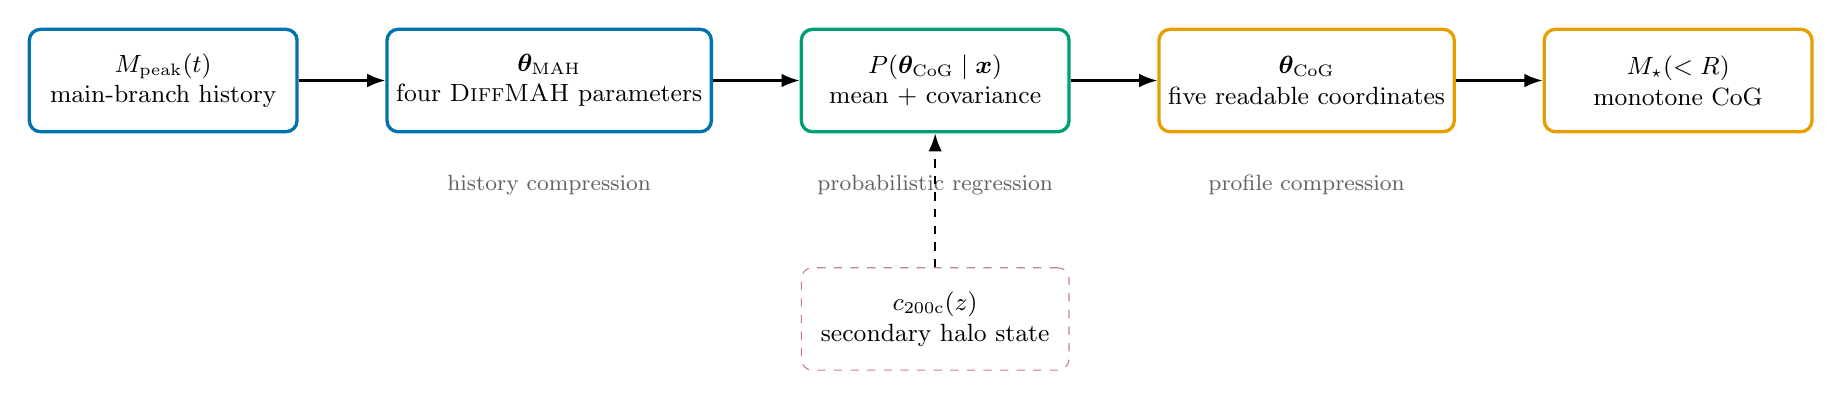
\begin{tikzpicture}[
      font=\small,
      node distance=8mm and 11mm,
      box/.style={draw,rounded corners,align=center,minimum height=13mm,minimum width=34mm,fill=white},
      arrow/.style={-{Latex[length=2.3mm]},thick},
      note/.style={align=center,font=\footnotesize,text=hsgray}
    ]
    \node[box,draw=hsblue,very thick] (mah) {$\Mpeak(t)$\\main-branch history};
    \node[box,draw=hsblue,very thick,right=of mah] (dmah) {$\vect{\theta}_{\rm MAH}$\\four \diffmah{} parameters};
    \node[box,draw=hsgreen,very thick,right=of dmah] (map) {$P(\vect{\theta}_{\cog}\mid\vect{x})$\\mean + covariance};
    \node[box,draw=hsorange,very thick,right=of map] (coords) {$\vect{\theta}_{\cog}$\\five readable coordinates};
    \node[box,draw=hsorange,very thick,right=of coords] (cog) {$M_\star(<R)$\\monotone CoG};
    \draw[arrow] (mah) -- (dmah);
    \draw[arrow] (dmah) -- (map);
    \draw[arrow] (map) -- (coords);
    \draw[arrow] (coords) -- (cog);
    \node[note,below=4mm of dmah] {history compression};
    \node[note,below=4mm of map] {probabilistic regression};
    \node[note,below=4mm of coords] {profile compression};
    \node[box,draw=hspurple,dashed,below=17mm of map] (conc) {$\ctwo(z)$\\secondary halo state};
    \draw[arrow,dashed] (conc) -- (map);
  \end{tikzpicture}
  }
  \caption{The direct conversion has three independently testable layers. A
  failure in profile compression, halo-to-coordinate prediction, or stochastic
  calibration should not be attributed to either of the other layers.}
  \label{fig:pipeline}
\end{figure}

\subsection{Monotone profile decoder}

For a predicted coordinate vector, the decoder constructs knots
$(\logten R_i,F_i)$ from the 2-kpc anchor, the three quantile radii, and the
outer boundary $(148.2\kpc,1)$. It uses a shape-preserving piecewise cubic
Hermite interpolator \citep{Fritsch1984}, clips the result to $0<F\leq1$, and
enforces cumulative monotonicity. The reconstructed profile is
\begin{equation}
  \logten\!\left[\frac{M_\star(<R)}{\Msun}\right]
  =\logten\!\left(\frac{M_{\star,\rm tot}}{\Msun}\right)
  +\logten F_\star(R).
  \label{eq:decoder}
\end{equation}
This decoder does not assume a Sersic, Moffat, or other global analytic profile
family. It assumes only the information in the five coordinates plus smooth,
monotone interpolation between their knots.

\subsection{Conditional mean and residual distribution}
\label{sec:emulator_math}

Let the halo feature vector be
\begin{equation}
  \vect{x}=(\logten M_p,u_c,\alpha_{\rm early},\alpha_{\rm late},\ctwo),
\end{equation}
and standardize each feature within the training sample,
\begin{equation}
  x_{s,j}=\frac{x_j-\overline{x}_j}{s_{x,j}}.
  \label{eq:standardization}
\end{equation}
The linear conditional mean uses
\begin{equation}
  \vect{\phi}_{\rm lin}(\vect{x}_s)=(1,x_{s,1},\ldots,x_{s,5}).
\end{equation}
The degree-2 model appends the seven terms selected in the earlier emulator
experiments,
\begin{align}
  \vect{\phi}_{2} = \big(&\vect{\phi}_{\rm lin},
  x_{\log M_p}^2,
  x_{u_c}x_{\alpha_{\rm late}},
  x_{\alpha_{\rm early}}^2,
  x_{\alpha_{\rm late}}x_{c},
  x_{\alpha_{\rm late}}^2,\nonumber\\
  &x_{\log M_p}x_{\alpha_{\rm early}},
  x_{\log M_p}x_{\alpha_{\rm late}}\big).
  \label{eq:poly2_basis}
\end{align}
For target coordinate $a$, the mean is
\begin{equation}
  \mu_a(\vect{x})=\vect{\beta}_a^{\mathsf T}\vect{\phi}(\vect{x}_s).
  \label{eq:mean_model}
\end{equation}

Scatter is allowed to vary from halo to halo. Its marginal variance is
\begin{equation}
  \sigma_a^2(\vect{x})=
  \exp\!\left[\vect{\gamma}_a^{\mathsf T}(1,\vect{x}_s)\right],
  \label{eq:heteroscedastic}
\end{equation}
with an $L_2$ penalty on the non-intercept variance slopes. A fixed residual
correlation matrix $\vect{C}$ couples the five coordinates, giving
\begin{equation}
  \vect{\Sigma}(\vect{x})=
  \operatorname{diag}[\vect{\sigma}(\vect{x})]\,
  \vect{C}\,
  \operatorname{diag}[\vect{\sigma}(\vect{x})].
  \label{eq:covariance}
\end{equation}
The working predictive model is therefore
\begin{equation}
  \vect{\theta}_{\cog}\mid\vect{x}
  \sim \mathcal{N}\!\left[\vect{\mu}(\vect{x}),\vect{\Sigma}(\vect{x})\right],
  \label{eq:conditional_gaussian}
\end{equation}
followed by the nonlinear monotone decoder in \cref{eq:decoder}. Gaussianity
applies in transformed coordinate space, not directly to stellar mass at each
radius.

\subsection{Prediction and evaluation statistics}
\label{sec:metrics}

All predictive comparisons are out of fold. For galaxy $i$ with $K=24$ CoG
radii, the conditional-mean profile error is summarized by
\begin{equation}
  \mathrm{RMS}_i=\left[\frac{1}{K}\sum_{k=1}^{K}
  \left(\widehat{m}_{ik}-m_{ik}\right)^2\right]^{1/2},
  \label{eq:profile_rms}
\end{equation}
where $m_{ik}=\logten[M_{\star,i}(<R_k)/\Msun]$. The report quotes the median
of $\mathrm{RMS}_i$ unless otherwise stated.

Probabilistic sharpness and calibration are measured with empirical CRPS
\citep{Gneiting2007}. For truth $y$ and $D$ draws $Y_d$,
\begin{equation}
  \widehat{\mathrm{CRPS}}(y)=
  \frac{1}{D}\sum_{d=1}^{D}|Y_d-y|
  -\frac{1}{2D^2}\sum_{d=1}^{D}\sum_{d'=1}^{D}|Y_d-Y_{d'}|.
  \label{eq:crps}
\end{equation}
The profile CRPS is averaged over galaxies and radii. Lower CRPS is better; it
rewards a distribution that is both concentrated and statistically calibrated.

Population comparisons use energy distance \citep{Szekely2013}. Because a
finite TNG sample compared with a resampled copy of itself has nonzero energy
distance, results are divided by this finite-sample floor. A ratio near unity
means the model population is statistically as close to TNG as two finite
realizations of the TNG population are to each other.

\section{Experiment 50: design at \texorpdfstring{$z=0.4$}{z=0.4}}
\label{sec:exp50_methods}

\ExpFifty{} is the controlled single-epoch test. It asks whether replacing PCA
profile coordinates with the readable vector in \cref{eq:exp50_coordinates}
changes either the compression accuracy or the held-out halo-to-profile
prediction. The sample contains 2539 galaxies, and every comparison uses the
same five galaxy folds and 32 stochastic draws per halo.

\subsection{Why the tests are separated}

\Cref{tab:exp50_tests} lists the motivation of each test. The ordering is
deliberate. The profile representation is validated before a halo relation is
fitted; the conditional mean is validated before stochastic population
properties are interpreted; and assembly claims require mass-conditioned null
controls.

\begin{longtable}{@{}p{0.20\textwidth}p{0.29\textwidth}p{0.43\textwidth}@{}}
  \caption{Logic of the \ExpFifty{} tests.}\label{tab:exp50_tests}\\
  \toprule
  Test & Motivation & What would constitute failure? \\
  \midrule
  \endfirsthead
  \toprule
  Test & Motivation & What would constitute failure? \\
  \midrule
  \endhead
  CoG compression & Establish whether five readable numbers preserve the
  measured profile independently of any halo model. & Reconstruction error
  comparable to the halo-prediction error, or a systematic central/outer bias.\\
  Central $f_2$ anchor & Quantile radii describe where broad fractions of mass
  lie but need not preserve the innermost aperture. & Accurate outer profile
  with a biased 2-kpc mass.\\
  Add $R_{90}$ & Test whether a more accurate coordinate system is also more
  predictable from the selected halo variables. & Improved reconstruction but
  unchanged or worse held-out prediction.\\
  PCA parity & Determine whether interpretability costs measurable predictive
  performance. & Readable-map CRPS difference larger than the empirical
  fold-to-fold variation of the PCA score.\\
  Final-mass-only control & Establish the baseline scalar SHMR information. &
  No improvement after adding assembly variables.\\
  MAH-shuffle control & Test whether the galaxy is using its own halo's MAH
  shape, rather than extra marginal flexibility. & Shuffling MAH shape within
  narrow final-mass bins leaves the score unchanged.\\
  Concentration shuffle & Test whether $\ctwo$ adds information beyond
  \diffmah{}. & Real and mass-conditioned shuffled concentration perform alike.\\
  Correlated draws & Test whether the conditional distribution reproduces the
  population, not only paired conditional means. & Draws do not improve the
  mass--size and central--outer population planes.\\
  Symbolic residual search & Ask whether a few stable nonlinear terms recover
  the gain of a dense quadratic relation. & Fold-specific expressions or a
  negligible end-to-end profile improvement.\\
  Concentration history & Test whether earlier $\ctwo$ measurements add
  information beyond current $\ctwo$. & Real histories do not outperform a
  mass-conditioned shuffled-history control.\\
  \bottomrule
\end{longtable}

\subsection{Compression candidates}

Three representations are compared on the measured profiles themselves:
\begin{enumerate}
  \item the adopted five-coordinate vector with $R_{20},R_{50},R_{80}$;
  \item a six-coordinate extension that also contains $R_{90}$;
  \item total stellar mass plus three PCA shape components.
\end{enumerate}
For PCA, total mass is separated from the shape
$\logten M_\star(<R)-\logten M_{\star,\rm tot}$ before computing the basis. The
in-sample reconstruction comparison is a compression floor, not a predictive
score. In the held-out comparison, the PCA mean shape, basis, halo regression,
and residual distribution are all fitted using only the training fold.

\subsection{Mean models and parity gate}

The linear and seven-term degree-2 means are those in
\cref{eq:mean_model,eq:poly2_basis}. The readable representation is declared
competitive if
\begin{equation}
  \mathrm{CRPS}_{\rm readable}-\mathrm{CRPS}_{\rm PCA}
  \leq s_{\rm fold,PCA},
  \label{eq:exp50_gate}
\end{equation}
where $s_{\rm fold,PCA}$ is the standard deviation of the five PCA fold scores.
This is a practical parity criterion, not a formal equivalence test. It asks
whether the difference between coordinate systems is smaller than the measured
partition sensitivity of the reference score.

\subsection{Assembly and concentration controls}

The main feature sets are
\begin{align}
  \vect{x}_{M} &= (\logten M_p),\\
  \vect{x}_{\rm MAH} &= (\logten M_p,u_c,\alpha_{\rm early},\alpha_{\rm late}),\\
  \vect{x}_{\rm full} &= (\vect{x}_{\rm MAH},\ctwo).
\end{align}
For the MAH null, $(u_c,\alpha_{\rm early},\alpha_{\rm late})$ are permuted
together among halos in ten narrow $\logten M_p$ bins. The mass distribution
and covariance among the shuffled MAH-shape variables are preserved, but their
pairing with the correct galaxy is destroyed. Concentration is tested with an
analogous within-mass-bin permutation. Consequently, a real-versus-shuffled
difference measures predictive information in the object-level pairing at
approximately fixed final mass; it does not by itself prove a causal effect.

\subsection{Symbolic regression protocol}

Symbolic regression is applied to residuals of the full linear model, rather
than replacing the linear relation. This ensures that a failed search cannot
erase a well-measured first-order dependence. PySR searches a restricted set of
algebraic corrections \citep{Cranmer2023}. The search is repeated independently
inside each training fold, and a candidate term is retained only if it appears
in at least four of five folds. The final judgment is the held-out profile CRPS
after decoding, not the symbolic training loss or the visual simplicity of an
expression.

\subsection{Concentration-history extension}

The gated extension uses the 2366-galaxy overlap with $\ctwo$ measured at
$z=(0.4,0.7,1.0,1.5,2.0)$. It compares current concentration, the complete
five-epoch concentration vector, and histories shuffled within final-mass bins.
The same folds and profile target are retained.


\section{Experiment 50: results}
\label{sec:exp50_results}

\subsection{The five readable coordinates preserve the measured CoG}

Without the 2-kpc fraction, the three quantile radii reproduce the CoG outside
roughly 5 kpc but leave the first measured aperture weakly constrained. Adding
$f_2$ lowers the median profile reconstruction RMS from $0.027\dex$ to
$0.00437\dex$. The adopted readable representation is $0.00100\dex$ worse than
the three-component PCA representation, whose median reconstruction RMS is
$0.00337\dex$, but both floors are more than an order of magnitude below the
halo-to-galaxy prediction error.

Adding $R_{90}$ lowers the readable reconstruction RMS to $0.00316\dex$, which
is $0.00021\dex$ better than PCA. It nevertheless changes held-out linear
profile CRPS from $0.06577\dex$ for the adopted five-coordinate representation
to $0.06601\dex$ for the six-coordinate version, making prediction worse by
$0.00023\dex$. The outermost additional coordinate is measurable from the CoG
but not sufficiently predictable from the available halo variables to improve
the reconstructed profile.

\begin{figure}[htbp]
  \centering
  \includegraphics[width=0.96\textwidth]{figures/exp50_representation.pdf}
  \caption{\ExpFifty{} representation study. The radial reconstruction errors
  and direct profile examples separate the information retained by each
  coordinate system from the later halo-prediction problem. The central-fraction
  coordinate is required to anchor the first measured aperture.}
  \label{fig:exp50_representation}
\end{figure}

\subsection{The readable halo-to-CoG map passes the PCA parity test}

The degree-2 readable model has held-out profile CRPS $0.06327\dex$. The
like-for-like degree-2 PCA reference has $0.06317\dex$. Thus the readable model
is worse by $0.00010\dex$, while the measured standard deviation among the five
PCA fold scores is $0.00024\dex$. It passes the gate in
\cref{eq:exp50_gate}.

The conditional-mean median profile RMS is $0.08560\dex$ for the readable model
and $0.08377\dex$ for PCA, so PCA is better by $0.00182\dex$ under this paired
mean statistic. The median largest fractional stellar-mass error beyond 5 kpc
is 24.64 per cent for the readable model and 24.25 per cent for PCA, making the
readable map worse by 0.39 percentage points. These small differences support
practical parity, not exact identity.

\begin{table}[htbp]
  \centering
  \caption{Held-out \ExpFifty{} prediction metrics. CRPS and RMS are in dex;
  lower values are better. Annular columns give RMS for CoG-derived stellar
  masses.}
  \label{tab:exp50_prediction}
  \resizebox{\textwidth}{!}{%
  \begin{tabular}{@{}lrrrrrr@{}}
    \toprule
    Model & Profile CRPS & Median profile RMS & $M(<10)$ & $M(10$--$30)$ & $M(30$--$50)$ & $M(50$--$100)$ \\
    \midrule
    Readable linear & 0.06577 & 0.08693 & 0.1168 & 0.1560 & 0.1717 & 0.1739 \\
    Readable degree-2 & 0.06327 & 0.08560 & 0.1115 & 0.1524 & 0.1670 & 0.1665 \\
    PCA linear & 0.06596 & 0.08631 & 0.1158 & 0.1555 & 0.1690 & 0.1697 \\
    PCA degree-2 & 0.06317 & 0.08377 & 0.1106 & 0.1513 & 0.1637 & 0.1667 \\
    \bottomrule
  \end{tabular}}
\end{table}

\begin{figure}[htbp]
  \centering
  \includegraphics[width=0.96\textwidth]{figures/exp50_predictive_skill.pdf}
  \caption{Held-out predictive comparison in \ExpFifty{}. The readable and PCA
  representations are evaluated on identical galaxy folds. The figure includes
  profile-wide scores and radial diagnostics; a low aggregate score is not used
  as a substitute for inspecting the reconstructed curves.}
  \label{fig:exp50_predictive_skill}
\end{figure}

\subsection{Total mass is much more predictable than detailed shape}

For the adopted degree-2 map, the held-out fraction of target-coordinate
variance explained is approximately 0.87 for total stellar mass, 0.31 for the
2-kpc fraction, 0.36 for $R_{20}$, 0.31 for the transformed $R_{20}$--$R_{50}$
gap, and 0.15 for the transformed $R_{50}$--$R_{80}$ gap. Therefore, the
selected halo variables tightly constrain overall stellar mass but only partly
constrain the radial mass distribution. A deterministic map would suppress
real profile diversity.

\begin{figure}[htbp]
  \centering
  \includegraphics[width=0.96\textwidth]{figures/exp50_parameter_predictions.pdf}
  \caption{Truth-versus-prediction and residual behavior for the five readable
  coordinates. The contrast between total-mass predictability and profile-shape
  predictability motivates treating the conversion as a conditional
  distribution.}
  \label{fig:exp50_parameters}
\end{figure}

\subsection{Assembly history and concentration both add paired information}

A final-mass-only linear model has median profile RMS $0.10890\dex$. Adding the
four \diffmah{} parameters lowers it to $0.09362\dex$, an improvement of
$0.01527\dex$. Shuffling the three MAH-shape variables at fixed final mass gives
$0.09472\dex$, which is $0.00109\dex$ worse than the correctly paired \diffmah{}
model. This is a modest but nonzero object-level assembly signal.

Adding correctly paired $z=0.4$ concentration lowers median profile RMS from
$0.09362\dex$ for \diffmah{} alone to $0.08693\dex$, an improvement of
$0.00669\dex$. Shuffling concentration within final-mass bins gives
$0.09338\dex$, nearly returning to the \diffmah{}-only reference. Concentration
therefore supplies information not encoded by the adopted smooth MAH
parameters.

\begin{figure}[htbp]
  \centering
  \includegraphics[width=0.96\textwidth]{figures/exp50_mass_binned_predictions.pdf}
  \caption{Measured and predicted CoGs with residuals in halo-mass bins at
  $z=0.4$. The conditional mean reproduces median trends but leaves broad
  object-to-object residuals, especially toward small radii.}
  \label{fig:exp50_mass_binned}
\end{figure}

\subsection{Correlated draws are required to reproduce the population}

The conditional mean is narrower than the TNG galaxy population. In the total
stellar mass--$R_{50}$ plane, its energy distance is 3.94 times the finite-sample
floor. One correlated draw per halo reduces the ratio to 1.35, making the draw
population 2.9 times closer to the floor under this ratio. In the central
$M_\star(<10\kpc)$ versus outer $M_\star(50$--$100\kpc)$ plane, the ratio falls
from 3.46 for the mean to 1.21 for a draw, again a 2.9-fold improvement. The
scatter model is thus necessary to represent the galaxy population.

The nominal 68 and 90 per cent pointwise intervals contain the measured CoGs
65.2 and 85.6 per cent of the time. The corresponding PCA coverages are 64.8
and 84.9 per cent. Both models are modestly under-covering, and 32 Monte Carlo
draws limit the precision of the tail estimates. The comparison does not reveal
a readable-coordinate-specific calibration failure.

\begin{figure}[htbp]
  \centering
  \includegraphics[width=0.96\textwidth]{figures/exp50_population_planes.pdf}
  \caption{Population-level validation in \ExpFifty{}. Conditional means
  collapse part of the intrinsic distribution, whereas correlated stochastic
  draws restore most of the observed width in mass--size and central--outer
  mass planes. Each population uses its own derived size.}
  \label{fig:exp50_population}
\end{figure}

\subsection{Symbolic regression finds useful corrections, but not a law}

The full linear map has profile CRPS $0.06577\dex$. Adding only nonlinear terms
that recur in at least four of five training folds lowers CRPS to
$0.06421\dex$, a 2.38 per cent improvement relative to linear. The dense
degree-2 model reaches $0.06327\dex$, a 3.80 per cent improvement; the sparse
terms therefore recover about 62 per cent of the available nonlinear gain.

The recurring standardized-variable terms are $c^2$ for total stellar mass,
$u_c\alpha_{\rm early}$ for the central fraction, and
$(\logten M_p)\alpha_{\rm early}$ for the middle radial gap. No correction
recurs in four folds for $R_{20}$ or the outer radial gap. Their coefficients
depend on the training-fold standardization, so these are empirical hypotheses,
not unit-independent physical equations.

\begin{figure}[htbp]
  \centering
  \includegraphics[width=0.96\textwidth]{figures/exp50_symbolic_regression.pdf}
  \caption{Nested-fold symbolic-regression result at $z=0.4$. Term recurrence
  is used as a stability filter, while the decoded held-out profile CRPS is the
  final criterion.}
  \label{fig:exp50_symbolic}
\end{figure}

\subsection{Concentration history adds a small independent signal}

On the 2366-galaxy overlap sample, the current-concentration degree-2 model has
profile CRPS $0.06318\dex$. Adding the five-epoch concentration history lowers
it to $0.06135\dex$, a 2.89 per cent improvement. Shuffling those histories
within final-mass bins gives $0.06325\dex$, which is 0.12 per cent worse than
the current-concentration reference. The real-history gain has the same sign
in all five held-out folds, whereas the shuffled history is worse in all five.

\begin{figure}[htbp]
  \centering
  \includegraphics[width=0.96\textwidth]{figures/exp50_concentration_history.pdf}
  \caption{Concentration-history extension in \ExpFifty{}. The real history is
  compared with current concentration and with histories permuted among halos
  of similar final mass. The gain is small but is not reproduced by the null.}
  \label{fig:exp50_concentration}
\end{figure}

\subsection{What \ExpFifty{} established}

At $z=0.4$, readable CoG coordinates can replace PCA coordinates without a
measurable loss at the precision of the five-fold comparison. The result is
probabilistic: only total stellar mass is tightly determined, and correlated
scatter is essential. Both MAH shape and concentration provide independent,
shuffle-controlled predictive information. The experiment does not establish
that one fixed relation applies at other epochs, that future halo history is
unnecessary, or that the sparse nonlinear terms are universal. Those questions
motivate \ExpFiftyOne{}.

\FloatBarrier


\section{Experiment 51: design across redshift}
\label{sec:exp51_methods}

\ExpFiftyOne{} extends the direct conversion to five epochs and asks whether it
can be made portable. Its tests are ordered from mechanical representation
checks to increasingly strong predictive claims. The main sample contains 2395
galaxies; the epoch-local and concentration analyses use the 2365-galaxy common
sample. All model comparisons use five held-out galaxy folds and 32 stochastic
draws unless stated otherwise.

\subsection{Why the CoG coordinates changed}

A small development subset did not contain the most compact valid object in the
full five-epoch sample. During the full-sample representation preflight, one
$z=2$ galaxy was found to contain 81.1 per cent of its measured stellar mass
inside 2 kpc. Its ordinary $R_{20}$ and $R_{50}$ are both below the first radial
grid point. Assigning $R_{20}=R_{50}=2\kpc$ would violate strict ordering;
discarding the object would remove exactly the type of compact galaxy the model
must retain.

The outer-mass definition in \cref{eq:outer_level,eq:exp51_coordinates} solves
this measurement problem without adding a parametric inner profile. The first
coordinate still fixes the 2-kpc fraction, while the other three radii describe
the resolved distribution of the remaining mass. The representation is
revalidated independently at every epoch before fitting any halo relation.

\subsection{Independent single-epoch ceilings}

At each redshift, the readable linear and degree-2 models are fitted
independently and compared with a three-component PCA model on identical folds.
The readable representation passes an epoch if
\begin{equation}
  \mathrm{CRPS}_{\rm readable}(z)-\mathrm{CRPS}_{\rm PCA}(z)
  \leq s_{\rm fold,PCA}(z).
  \label{eq:exp51_parity_gate}
\end{equation}
This stage answers whether a direct map is feasible at each snapshot. It does
not yet assert that one relation evolves smoothly with redshift.

At $z=2$, additional controls compare final descendant mass alone, concurrent
halo mass alone, complete descendant \diffmah{}, shuffled descendant MAH shape,
and complete descendant \diffmah{} plus concentration. These controls reveal
whether a superficially rich final-descendant feature vector is actually more
informative than the halo mass at the correct epoch.

\subsection{Descendant-conditioned and epoch-local maps}
\label{sec:two_scopes}

The two prediction scopes are shown in \cref{fig:information_boundary}. For a
population selected at $z=0.4$, the descendant-conditioned relation is
\begin{equation}
  P\!\left[\vect{\theta}_{\cog}(z)\given
  \vect{\theta}_{\rm MAH}^{\,z=0.4},\ctwo(z=0.4)\right].
  \label{eq:descendant_map}
\end{equation}
The complete history is a property of the selected descendant, even when the
target is its earlier progenitor. This model is useful for reconstructing
histories of a low-redshift-selected sample.

For an independently selected catalog at redshift $z$, the portable relation is
\begin{equation}
  P\!\left[\vect{\theta}_{\cog}(z)\given
  \vect{\theta}_{\rm MAH}^{\,\leq t_z;t_z},\ctwo(z)\right],
  \label{eq:local_map}
\end{equation}
where \diffmah{} is fitted only to $t\leq t_z$ and anchored at $t_z$. The
notation $\leq t_z;t_z$ states both the data boundary and the fit endpoint.

\begin{figure}[htbp]
  \centering
  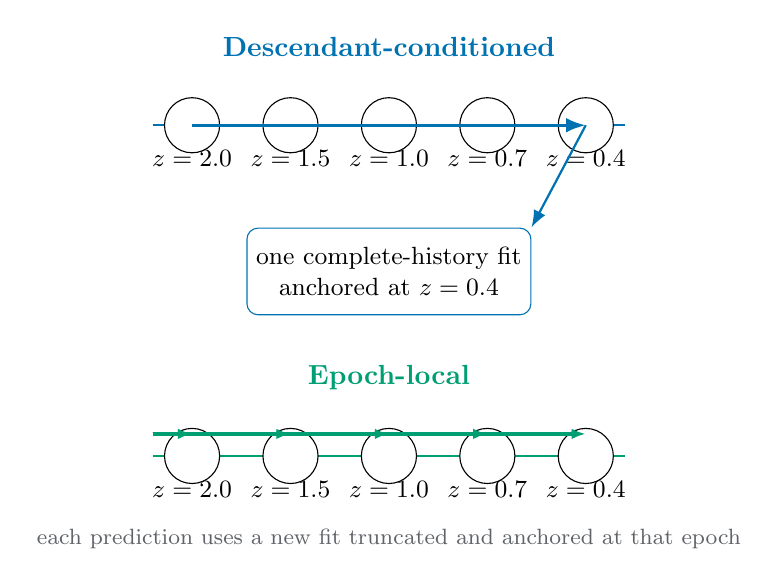
\begin{tikzpicture}[
      font=\small,
      epoch/.style={circle,draw,minimum size=7mm,inner sep=0pt},
      box/.style={draw,rounded corners,align=center,minimum height=11mm,minimum width=34mm},
      arrow/.style={-{Latex[length=2.2mm]},thick}
    ]
    \node[font=\bfseries,hsblue] at (0,2.2) {Descendant-conditioned};
    \draw[thick,hsblue] (-3,1.2) -- (3,1.2);
    \foreach \x/\z in {-2.5/2.0,-1.25/1.5,0/1.0,1.25/0.7,2.5/0.4}{
      \node[epoch,fill=white] (d\x) at (\x,1.2) {};
      \node[below=2mm] at (\x,1.2) {$z=\z$};
    }
    \draw[very thick,hsblue,-{Latex[length=2.5mm]}] (-2.5,1.2) -- (2.5,1.2);
    \node[box,draw=hsblue,below=13mm] (dfit) at (0,1.2) {one complete-history fit\\anchored at $z=0.4$};
    \draw[arrow,hsblue] (2.5,1.2) -- (dfit.north east);

    \node[font=\bfseries,hsgreen] at (0,-2.0) {Epoch-local};
    \draw[thick,hsgreen] (-3,-3.0) -- (3,-3.0);
    \foreach \x/\z in {-2.5/2.0,-1.25/1.5,0/1.0,1.25/0.7,2.5/0.4}{
      \node[epoch,fill=white] at (\x,-3.0) {};
      \node[below=2mm] at (\x,-3.0) {$z=\z$};
      \draw[very thick,hsgreen,-{Latex[length=1.8mm]}] (-3,-2.72) -- (\x,-2.72);
    }
    \node[align=center,font=\footnotesize,text=hsgray] at (0,-4.05)
      {each prediction uses a new fit truncated and anchored at that epoch};
  \end{tikzpicture}
  \caption{Information boundary in \ExpFiftyOne{}. The descendant-conditioned
  model may use later growth because the population is selected by its final
  descendants. The epoch-local model is restricted to information available by
  each prediction epoch and is the portable form of the conversion.}
  \label{fig:information_boundary}
\end{figure}

The official halo history is truncated at every epoch and fitted for every
galaxy with $t\geq1\gyr$. This produces $2365\times5=11825$ epoch-local
\diffmah{} fits. A current-halo-mass-only baseline and mass-conditioned MAH-shape
and concentration shuffles are repeated at each snapshot.

\subsection{Held-epoch coefficient closure}

Smooth-looking coefficient curves are not sufficient evidence for a
continuous-redshift model. For each interior epoch, that epoch is omitted, the
descendant-conditioned relation is fitted at the other four snapshots, and its
coefficients are interpolated quadratically to the missing redshift. The
interpolated prediction is compared with both a direct fit and the nearest
available snapshot. The predeclared criterion is
\begin{equation}
  \frac{\mathrm{CRPS}_{\rm interp}(z)}
       {\mathrm{CRPS}_{\rm direct}(z)}-1 < 0.05.
  \label{eq:closure_gate}
\end{equation}
Because the descendant features are identical at all target epochs, one
training-fold feature standardization is meaningful across this test. The same
procedure cannot yet be transferred mechanically to the epoch-local features,
whose distributions and physical anchors evolve with redshift.

\subsection{Concentration at the correct epoch}

With descendant \diffmah{} held fixed, three concentration descriptions are
compared: $\ctwo(z=0.4)$, concurrent $\ctwo(z)$, and all earlier concentration
measurements available by $z$. Concurrent and historical concentration values
are separately shuffled within concurrent halo-mass bins. This identifies
information in the halo--galaxy pairing rather than improvement caused solely
by extra columns or their marginal distributions.

\subsection{Temporal residual coherence}
\label{sec:ar1}

Independent snapshot draws would produce discontinuous individual histories,
while reusing one residual vector at all epochs would make histories too
persistent. The out-of-fold coordinate residuals are standardized and their
cross-epoch correlation is summarized by
\begin{equation}
  \operatorname{Corr}(\epsilon_{a,i},\epsilon_{a,j})
  \approx \rho^{|i-j|},
  \label{eq:ar1}
\end{equation}
where $a$ indexes a profile coordinate and $i,j$ index the ordered snapshots.
The fitted scalar $\rho$ is used to draw an AR(1)-in-epoch latent sequence, while
the within-epoch coordinate covariance retains the model in
\cref{eq:covariance}. Coherence is judged using the Spearman rank correlation
of total mass, $R_{50}$, and $f_2$ between snapshots. This tests galaxy histories
directly; no collection of single-epoch scores can replace it.

\subsection{Symbolic transfer at \texorpdfstring{$z=2$}{z=2}}

The final stage repeats the nested-fold residual symbolic search using only the
epoch-local $z=2$ inputs. Four models are compared: linear, the three stable
$z=0.4$ terms, a new $z=2$ symbolic search, and the dense degree-2 relation.
The purpose is not to maximize the symbolic search budget. It is to test whether
the low-complexity nonlinear structure discovered at $z=0.4$ transfers to a
different epoch and input definition.

\section{Experiment 51: results}
\label{sec:exp51_results}

\subsection{The high-redshift-safe coordinates remain accurate}

\Cref{tab:representation_redshift} shows the median RMS between each measured
CoG and its reconstruction from five coordinates. The readable error remains
between $0.00367$ and $0.00415\dex$ across all five snapshots. PCA is better by
$0.00018$--$0.00059\dex$, but both representations remain far below the
halo-to-profile prediction error. The central-censored coordinates therefore
solve the unresolved-radius problem without materially degrading compression.

\begin{table}[htbp]
  \centering
  \caption{Median full-CoG reconstruction RMS in dex. Lower is better. These
  are representation floors, not held-out halo predictions.}
  \label{tab:representation_redshift}
  \begin{tabular}{@{}lrrrrr@{}}
    \toprule
    Representation & $z=0.4$ & $z=0.7$ & $z=1.0$ & $z=1.5$ & $z=2.0$ \\
    \midrule
    Readable outer-mass coordinates & 0.00369 & 0.00367 & 0.00392 & 0.00415 & 0.00408 \\
    PCA, three components & 0.00334 & 0.00339 & 0.00374 & 0.00385 & 0.00349 \\
    \bottomrule
  \end{tabular}
\end{table}

\subsection{The readable map remains competitive with PCA}

\Cref{tab:parity_redshift} gives the held-out profile CRPS. At every epoch the
readable degree-2 model is slightly worse than PCA, by $0.00018$--$0.00070\dex$.
Each difference is smaller than the measured PCA fold-to-fold standard
deviation at that epoch, $0.00117$--$0.00333\dex$. The readable map therefore
passes the predefined parity gate at all five snapshots.

\begin{table}[htbp]
  \centering
  \caption{Five-fold held-out descendant-conditioned profile CRPS in dex.
  Lower is better. $\Delta$ is readable minus PCA, so positive values favor
  PCA.}
  \label{tab:parity_redshift}
  \begin{tabular}{@{}lrrrrr@{}}
    \toprule
    Quantity & $z=0.4$ & $z=0.7$ & $z=1.0$ & $z=1.5$ & $z=2.0$ \\
    \midrule
    Readable degree-2 & 0.06253 & 0.06651 & 0.07236 & 0.08067 & 0.09354 \\
    PCA degree-2 & 0.06223 & 0.06618 & 0.07167 & 0.08050 & 0.09294 \\
    $\Delta$ & 0.00030 & 0.00033 & 0.00070 & 0.00018 & 0.00060 \\
    PCA fold standard deviation & 0.00181 & 0.00169 & 0.00117 & 0.00261 & 0.00333 \\
    \bottomrule
  \end{tabular}
\end{table}

Nonlinearity becomes increasingly important toward high redshift. Relative to
the readable linear model, the degree-2 mean lowers profile CRPS by 3.42 per
cent at $z=0.4$, 8.33 per cent at $z=0.7$, 16.40 per cent at $z=1$, 21.63 per
cent at $z=1.5$, and 21.47 per cent at $z=2$. The stable profile coordinates do
not imply a redshift-independent linear halo relation.

\begin{figure}[htbp]
  \centering
  \includegraphics[width=0.98\textwidth]{figures/exp51_redshift_summary.pdf}
  \caption{Summary of the descendant-conditioned five-epoch experiment.
  Panel A tests only the CoG representation; panel B compares held-out
  probabilistic prediction; panel C illustrates coefficient evolution; panel D
  tests interpolation after removing an entire epoch.}
  \label{fig:exp51_summary}
\end{figure}

\subsection{Concurrent halo mass is a stronger high-redshift baseline}

At $z=2$, the final-descendant-mass-only model has a median
conditional-mean profile RMS of $0.18255\dex$. Concurrent $z=2$ halo mass alone lowers this to
$0.12501\dex$, an improvement of $0.05754\dex$. Complete descendant \diffmah{}
without concentration gives $0.13315\dex$, worse than concurrent mass alone by
$0.00814\dex$. Shuffling descendant MAH shape gives $0.18400\dex$, close to the
final-descendant-mass baseline. Adding $z=0.4$ concentration to descendant
\diffmah{} lowers the error to $0.13028\dex$ but does not overtake concurrent
mass. These controls warn that ``more history'' is not automatically a better
feature description when its normalization belongs to the wrong epoch.

\begin{figure}[htbp]
  \centering
  \includegraphics[width=0.98\textwidth]{figures/exp51_z2_predictions.pdf}
  \caption{Descendant-conditioned $z=2$ predictions in three concurrent
  halo-mass bins. Top panels compare median CoGs; bottom panels show the median
  fractional conditional-mean residual and its 16th--84th percentile range.
  Median trends can be accurate while individual residuals remain broad.}
  \label{fig:exp51_z2_descendant}
\end{figure}

\subsection{Descendant-conditioned coefficients pass held-epoch closure}

At $z=0.7$, $1.0$, and $1.5$, direct-fit CRPS is $0.06651$, $0.07236$, and
$0.08067\dex$. Interpolating coefficients without fitting the held epoch gives
$0.06733$, $0.07267$, and $0.08160\dex$, which is worse by only 1.23, 0.43, and
1.15 per cent. All pass the 5 per cent gate in \cref{eq:closure_gate}. Copying
the nearest available epoch gives $0.07530$, $0.08198$, and $0.10665\dex$, which
is substantially worse than interpolation.

This result establishes a continuous-redshift route for the
descendant-conditioned feature definition. It does not establish closure for
epoch-local inputs, because their normalizations and distributions change with
the fitting endpoint.

\begin{figure}[htbp]
  \centering
  \includegraphics[width=0.98\textwidth]{figures/exp51_coefficient_evolution.pdf}
  \caption{Evolution of the fitted standardized linear coefficients for all
  five readable profile coordinates. The figure is descriptive; the actual
  evidence for redshift continuity is the held-epoch predictive test, not the
  visual smoothness of these lines.}
  \label{fig:exp51_coefficients}
\end{figure}

\subsection{Epoch-local \diffmah{} is feasible and stronger at high redshift}

All 2365 galaxies receive valid \diffmah{} fits at all five truncation epochs.
The 11825 fits take 37.86 seconds in the measured run. Median mass-history
reconstruction RMS decreases from $0.0707\dex$ for fits ending at $z=0.4$ to
$0.0505\dex$ for fits ending at $z=2$. This decrease partly reflects the shorter
high-redshift fitted interval and must not be interpreted as stronger parameter
identification.

\Cref{tab:local_crps} compares the models using profile CRPS. Adding local
\diffmah{} and concurrent concentration lowers CRPS by 20.79--25.41 per cent
relative to concurrent halo mass alone. At $z=1.5$ and $z=2$, the local model
has CRPS $0.07197$ and $0.08363\dex$, compared with $0.07847$ and
$0.09107\dex$ for complete descendant \diffmah{} with the same concurrent
concentration. The epoch-local model is better by 8.28 and 8.17 per cent. The
high-redshift predictive signal therefore does not depend on access to later
halo growth.

\begin{table}[htbp]
  \centering
  \caption{Held-out profile CRPS in dex for the epoch-local analysis. Lower is
  better. The local model uses only history available by the listed epoch.}
  \label{tab:local_crps}
  \resizebox{\textwidth}{!}{%
  \begin{tabular}{@{}lrrrrr@{}}
    \toprule
    Model & $z=0.4$ & $z=0.7$ & $z=1.0$ & $z=1.5$ & $z=2.0$ \\
    \midrule
    Concurrent halo mass only & 0.08434 & 0.08266 & 0.08788 & 0.09649 & 0.11084 \\
    Local \diffmah{} & 0.07091 & 0.07186 & 0.07500 & 0.07928 & 0.09174 \\
    Local \diffmah{} + concurrent $c$ & 0.06443 & 0.06548 & 0.06726 & 0.07197 & 0.08363 \\
    Local MAH shape shuffled & 0.06806 & 0.07013 & 0.07381 & 0.08141 & 0.09881 \\
    Local concentration shuffled & 0.06798 & 0.06930 & 0.07148 & 0.07577 & 0.08670 \\
    Descendant \diffmah{} + concurrent $c$ & 0.06310 & 0.06430 & 0.06887 & 0.07847 & 0.09107 \\
    \bottomrule
  \end{tabular}}
\end{table}

The real pairing between a galaxy and its MAH shape becomes more valuable with
redshift. Relative to concurrent mass alone, real local \diffmah{} plus
concentration improves CRPS by 23.60 percentage points at $z=0.4$ and 24.55
points at $z=2$. When MAH shape is shuffled at fixed concurrent mass, the
improvements are only 19.29 and 10.85 points. The additional value of the real
pairing is therefore 4.31 percentage points at $z=0.4$ and 13.69 points at
$z=2$. The analogous real-versus-shuffled concentration contribution is 4.21
and 2.77 percentage points at those epochs.

\begin{figure}[htbp]
  \centering
  \includegraphics[width=0.98\textwidth]{figures/exp51_epoch_local.pdf}
  \caption{Epoch-local \diffmah{} analysis. Panel A reports the truncated-history
  fit error; panel B compares portable, descendant-conditioned, and control
  profile CRPS; panel C expresses the same comparisons as improvement relative
  to concurrent halo mass.}
  \label{fig:exp51_local}
\end{figure}

\begin{figure}[htbp]
  \centering
  \includegraphics[width=0.98\textwidth]{figures/exp51_epoch_local_z2_predictions.pdf}
  \caption{Direct profile validation of the portable $z=2$ model in three
  concurrent halo-mass bins. Median conditional-mean biases are generally a few
  per cent, while the broad residual bands show the much larger individual
  scatter represented by the stochastic model.}
  \label{fig:exp51_local_z2}
\end{figure}

\subsection{Concentration should be measured at the prediction epoch}

Holding descendant \diffmah{} fixed, replacing $z=0.4$ concentration with
concurrent concentration improves profile CRPS by 3.33 per cent at $z=0.7$,
4.66 per cent at $z=1$, 2.93 per cent at $z=1.5$, and 2.23 per cent at $z=2$.
Mass-conditioned shuffled concurrent concentrations are 0.10--2.30 per cent
worse than the $z=0.4$-concentration reference. The signal is therefore in the
correct halo--galaxy pairing and epoch label, not merely in adding one variable.

In a linear model, adding all concentration measurements available by the
prediction epoch improves on concurrent concentration by 3.40 per cent at
$z=0.4$ and 2.06 per cent at $z=0.7$, but by at most 0.17 per cent at $z\geq1$.
An extended concentration history is useful mainly when a substantial earlier
history is available.

\begin{figure}[htbp]
  \centering
  \includegraphics[width=0.98\textwidth]{figures/exp51_concentration_redshift.pdf}
  \caption{Concentration tests across redshift. Real concurrent concentration
  is compared with $z=0.4$ concentration and mass-conditioned shuffles. The
  final panel asks whether still earlier concentration values improve a linear
  model after concurrent concentration is known.}
  \label{fig:exp51_concentration}
\end{figure}

\subsection{The temporal residual model repairs over-coherent means}

The standardized held-out coordinate residuals yield $\rho=0.660$ in the AR(1)
approximation of \cref{eq:ar1}. For half-mass radius, the measured Spearman rank
correlation between $z=0.4$ and $z=2$ is 0.330. The conditional means have
correlation 0.591 and are therefore too persistent. The average correlation
among coherent stochastic draws is 0.228, which removes most of the excess but
undershoots the TNG value by 0.102.

For adjacent epoch pairs, TNG half-mass-radius correlations are 0.816, 0.819,
0.727, and 0.706. The coherent-draw averages are 0.787, 0.779, 0.712, and 0.630,
respectively. The single-$\rho$ model is a useful first approximation, but its
last adjacent pair and full-baseline persistence are too weak.

\begin{figure}[htbp]
  \centering
  \includegraphics[width=0.98\textwidth]{figures/exp51_cross_epoch_coherence.pdf}
  \caption{Cross-epoch residual and half-mass-radius rank correlations. The
  conditional mean is too coherent because regression suppresses individual
  scatter. AR(1)-coupled draws are much closer to TNG but slightly decorrelate
  the longest baseline too strongly.}
  \label{fig:exp51_coherence}
\end{figure}

\subsection{The symbolic corrections do not define a universal relation}

At $z=2$, the epoch-local linear model has profile CRPS $0.08804\dex$. The fixed
$z=0.4$ terms reach $0.08758\dex$, a 0.52 per cent improvement. A new nested
$z=2$ symbolic search reaches $0.08717\dex$, a 1.00 per cent improvement. The
dense degree-2 model reaches $0.08363\dex$, a 5.01 per cent improvement over
linear. Thus the new symbolic terms recover only about 20 per cent of the
available nonlinear gain.

No term recurs in four of five folds for total mass, $f_2$, or the outer radial
gap. A squared mass term recurs for $R_{20,\rm out}$; four coupled terms involving
mass, transition time, and growth index recur for the middle gap. This
target-specific structure is too complicated and too weak in decoded profile
performance to present as a compact redshift-independent law.

\begin{figure}[htbp]
  \centering
  \includegraphics[width=0.98\textwidth]{figures/exp51_symbolic_z2.pdf}
  \caption{Epoch-local symbolic residual test at $z=2$. The dense degree-2
  relation retains a clear predictive advantage over both transferred
  $z=0.4$ terms and a new stability-filtered symbolic search.}
  \label{fig:exp51_symbolic}
\end{figure}

\subsection{What \ExpFiftyOne{} established}

A readable, probabilistic conversion is viable at each tested snapshot and can
be made portable by refitting the halo assembly clock at the prediction epoch.
The high-redshift result is not an artifact of future halo information.
Descendant-conditioned coefficients pass an explicit redshift-interpolation
test, but continuous-redshift closure has not yet been demonstrated for the
epoch-local features. A simple temporal stochastic model is necessary and
approximately successful. No compact universal symbolic equation is supported.

\FloatBarrier

\section{Robustness and validity audit}
\label{sec:robustness}

The experiments contain several strong internal controls, but they do not have
the status of an external validation. This section separates what is directly
demonstrated from what remains conditional or suggestive.

\subsection{Cross-validation and leakage control}

All quoted predictive scores are out of fold. For the readable models, feature
standardization, mean coefficients, heteroscedastic variance coefficients, and
the residual correlation matrix are fitted using only the training galaxies.
For PCA, the mean profile, PCA basis, and halo-to-component regression are also
recomputed in each training fold. The symbolic searches are nested inside the
training folds. Thus neither a global PCA basis nor a globally selected symbolic
expression has access to the held-out targets.

The descendant-conditioned high-redshift model does contain halo growth after
the target epoch. This is not hidden leakage when the scientific sample is
defined by its known $z=0.4$ descendants, but it is an invalid feature set for
painting an independently selected high-redshift halo catalog. The epoch-local
test explicitly closes this information channel and improves the result at
$z\geq1$, which strengthens rather than weakens the main high-redshift claim.

\subsection{Null controls and the meaning of an assembly signal}

The final-mass and concurrent-mass baselines measure how much can be learned
without MAH shape. The within-mass-bin shuffles preserve the mass distribution
and approximately preserve the marginal distribution and internal covariance
of the shuffled feature block. They destroy its object-level association with
the galaxy. A real-versus-shuffled improvement is therefore evidence of
predictive assembly information at approximately fixed mass.

This design does not identify a causal intervention. MAH parameters can be
correlated with merger orbital structure, environment, concentration, or other
unmodeled variables. The appropriate statement is that the real halo history
contains predictive information for the galaxy profile that is lost when halo
histories are reassigned among similar-mass objects.

\subsection{Representation and sample-quality checks}

The CoG compression is tested before halo fitting and remains near $0.004\dex$
at every epoch. Invalid or dropped interpolation knots are counted. The full
sample, rather than only a development subset, is used for the representation
preflight. This step exposed the compact $z=2$ galaxy and caused the move to
outer-mass quantiles.

Two objects with broken progenitor matches are removed using the established
mass-drop criterion. This is a quality-control exclusion, not a model-dependent
outlier rejection. The report does not claim robustness to other possible
merger-tree failures that remain unidentified.

\subsection{Halo-history fitting}

The implementation in \cref{eq:diffmah_alpha,eq:diffmah_mass} is checked by
synthetic parameter recovery. Epoch-local fits use only $t\geq1\gyr$, consistent
with the regime where \diffmah{} is expected to approximate resolved halo
histories accurately \citep{Hearin2021}. All 2365 common-sample galaxies obtain
five finite successful fits. The median mass-history RMS is $0.0505$--$0.0707$
dex, but the fit parameters can still be covariant. These experiments evaluate
their predictive combination; they do not report full posterior uncertainties
for individual \diffmah{} parameters.

\subsection{Monte Carlo precision and calibration}

The empirical profile CRPS and coverage use 32 draws per galaxy. This is
adequate for the central distribution and efficient model comparisons, but
quantiles at 5 and 95 per cent are coarsely sampled. The similar undercoverage
of readable and PCA models suggests that it is not caused by the readable
coordinate choice. A publication-level calibration claim should repeat the
final model with more draws or use analytic coordinate-space intervals propagated
through a larger numerical sample.

The residual model is multivariate Gaussian in transformed coordinate space.
Non-Gaussian tails, multimodality, and mass-dependent correlations beyond the
adopted factorization can remain. The AR(1) temporal model uses one average
coefficient for all coordinates and epoch spacings. Its endpoint mismatch is
direct evidence that this approximation is incomplete.

\subsection{Symbolic-regression correction and rerun}

The first full $z=2$ symbolic run was invalid. Python's cached module name
selected the \ExpFifty{} decoder after the profiles had been compressed with
\ExpFiftyOne{} coordinates. Target labels in the direct prediction figure
exposed the inconsistency. That run was discarded; the import was made explicit
and the complete nested calculation was repeated. Only the corrected results in
\cref{fig:exp51_symbolic} and this report are retained. This incident illustrates
why decoded-profile inspection is a validity check rather than a presentation
step.

\subsection{Scope limitations}

The most important remaining limitations are:
\begin{itemize}
  \item one hydrodynamical simulation, with no resolution or subgrid-model
  comparison;
  \item a massive-central sample rather than a mass-complete galaxy population;
  \item one projected CoG per galaxy and no modeled observational errors;
  \item no external validation of the halo feature distributions or fitted
  coefficients;
  \item no explicit initial-condition, merger-orbit, satellite, or environment
  features;
  \item independent single-epoch epoch-local fits rather than a validated
  continuous-redshift portable model;
  \item a Gaussian residual family and a one-parameter temporal correlation
  model.
\end{itemize}

\subsection{Claim-strength summary}

\begin{longtable}{@{}p{0.36\textwidth}p{0.22\textwidth}p{0.34\textwidth}@{}}
  \caption{Strength and scope of the main claims.}\label{tab:claim_strength}\\
  \toprule
  Claim & Status & Qualification \\
  \midrule
  \endfirsthead
  \toprule
  Claim & Status & Qualification \\
  \midrule
  \endhead
  Five readable coordinates accurately reconstruct the measured CoG. &
  Mechanically demonstrated & Median representation RMS near $0.004\dex$ on
  the full retained samples.\\
  The readable map matches PCA predictive performance. & Supported within
  TNG300 & Difference is below PCA fold variation at all five epochs; this is
  practical parity, not formal statistical equivalence.\\
  MAH shape contains profile information beyond halo mass. & Supported within
  TNG300 & Real pairing outperforms mass-conditioned shuffled MAH shape.\\
  Concentration adds information beyond \diffmah{}. & Supported within TNG300 &
  Real concurrent concentration outperforms its mass-conditioned shuffle.\\
  Future halo growth is required for high-$z$ prediction. & Rejected by current
  test & Epoch-local inputs are better at $z=1.5$ and $z=2$.\\
  Descendant-conditioned coefficients can be interpolated in redshift. &
  Supported on fitted interval & All three held interior epochs pass the 5 per
  cent closure gate.\\
  Epoch-local coefficients define a continuous-$z$ model. & Not yet tested &
  Requires common physical scaling of evolving inputs and held-epoch closure.\\
  A one-parameter AR(1) residual process is exact. & Rejected as exact & It
  repairs over-coherence but undershoots the longest-baseline size correlation.\\
  A compact universal symbolic law has been discovered. & Not supported & The
  sparse $z=2$ gain is 1.00 per cent versus 5.01 per cent for dense degree-2.\\
  The map is causal or externally portable. & Not established & Requires other
  simulations, observational forward modeling, and a causal design.\\
  \bottomrule
\end{longtable}


\section{Combined interpretation}
\label{sec:interpretation}

\subsection{What the direct conversion now means}

The successful object is not a single equation that turns a halo history into
one deterministic galaxy profile. It is the composition
\begin{equation}
  \Mpeak(t),\ctwo(t)
  \longrightarrow \vect{x}(z)
  \longrightarrow P(\vect{\theta}_{\cog}\mid\vect{x},z)
  \longrightarrow P[M_\star(<R)\mid\vect{x},z].
  \label{eq:final_composition}
\end{equation}
The first arrow defines a compact halo state, the second is a fitted conditional
distribution, and the third is a monotone coordinate decoder. The model is
interpretable because its intermediate galaxy variables are total mass,
central fraction, and radial quantiles. It remains statistical because much of
the profile-shape variance is unresolved by the selected halo inputs.

\subsection{Why readable coordinates can match PCA}

PCA is optimized to reconstruct variance in the particular training sample.
The readable coordinates are instead chosen to preserve scientifically useful
functionals of a monotone cumulative profile. Their success indicates that, on
the adopted radial grid, the dominant profile variation can be captured by one
normalization, one central anchor, and three ordered outer scales. The result
does not imply that these are unique sufficient statistics. Adding $R_{90}$
improves the representation floor but not the halo prediction, demonstrating
that sufficiency for profile reconstruction and predictability from halos are
different requirements.

\subsection{Why the model must remain probabilistic}

The conditional mean predicts total stellar mass well but explains only
15--36 per cent of the variance in individual shape coordinates at $z=0.4$.
This remaining scatter is physically plausible: baryonic feedback, merger
orbits, satellite structure, stellar stripping, and projection need not be
fully determined by a smooth main-branch MAH and one concentration measurement.
The correlated residual distribution restores most of the population width
that the mean suppresses. Removing it would change the scientific model, not
merely its error bars.

\subsection{What the epoch-local result changes}

The strongest \ExpFiftyOne{} result is not simply that a $z=2$ fit succeeds. It
is that the fit improves when the halo assembly parameters are defined using
the correct epoch-local clock. Complete descendant \diffmah{} summarizes how a
halo reaches $z=0.4$; it is not automatically the most informative coordinate
system for the state of its progenitor at $z=2$. Re-anchoring the same class of
mass-history model at the prediction epoch aligns the mass normalization,
transition time, and growth indices with the target galaxy state.

The improvement also changes how ``portability'' should be described. The
functional form is portable in the sense that any halo with a resolved past
history can be compressed to four \diffmah{} parameters. The fitted
halo-to-galaxy coefficients are not yet externally portable: they have been
trained and tested only within TNG300.

\subsection{Relation to the deposition-and-migration model}

The direct conversion and the deposition model answer related but different
questions. The deposition model proposes an explicit history-to-radius
mechanism and can be interrogated in terms of when stellar mass arrives and
where it moves. Its assumptions are consequently more numerous and its
parameter degeneracies can be physically informative. The direct model asks
for the lowest-complexity conditional relation that preserves observable CoGs.
It has fewer mechanistic assumptions but does not identify a stellar mass flux
or migration trajectory.

The two models can therefore act as mutual controls. The direct map supplies a
statistical performance ceiling and reveals which profile coordinates contain
assembly information. The deposition model can test whether an explicit
phenomenological mechanism reproduces those dependencies and their redshift
evolution. Agreement on a dependence would be stronger evidence than either
model alone; disagreement would identify where mechanistic assumptions or
statistical shortcuts matter.

\subsection{Why symbolic regression did not yet deliver the hoped-for equation}

Symbolic regression is most useful when the relation is both low-dimensional
and stable under resampling. At $z=0.4$, three recurring residual corrections
recover a substantial fraction of the dense nonlinear gain. At $z=2$, the
nonlinearity is larger but is distributed across more target-specific terms,
and the $z=0.4$ terms transfer weakly. This pattern can arise if the natural
variables change with epoch, if interactions are genuinely numerous, or if a
small symbolic law is obscured by residual covariance and measurement noise.

The correct conclusion is not that symbolic regression is unsuitable. It is
that the current standardized variables and independent-epoch formulation do
not support a compact universal equation. A future search should follow, not
precede, construction of physically consistent epoch-local coordinates and an
explicit redshift variable.

\subsection{Priority of the next tests}

The next decisive analysis is held-epoch closure for the epoch-local model.
Because $\logten M_p$ and $u_c$ are anchored at different cosmic times, the
features require a common physical scaling before their coefficients can be
interpolated. A sensible sequence is:
\begin{enumerate}
  \item express local times relative to the cosmic age at prediction and masses
  relative to concurrent halo mass where appropriate;
  \item standardize with one training-set convention shared across epochs;
  \item remove each interior epoch and predict it from the others;
  \item test whether explicit low-order redshift terms retain the high-$z$
  degree-2 gain;
  \item replace the one-$\rho$ residual model only if a more flexible process
  measurably improves both adjacent and endpoint coherence;
  \item validate the frozen design in another simulation or resolution before
  library graduation.
\end{enumerate}


\section{Conclusions}
\label{sec:conclusions}

Experiments 50 and 51 support the central feasibility of a direct,
phenomenologically readable halo-to-stellar-profile conversion.

\begin{enumerate}
  \item At $z=0.4$, total stellar mass, the 2-kpc mass fraction, and three
  ordered enclosed-mass radii reconstruct the measured CoG with median error
  $0.00437\dex$.

  \item The readable degree-2 map reaches held-out profile CRPS
  $0.06327\dex$, compared with $0.06317\dex$ for a matched PCA model. Its
  $0.00010\dex$ disadvantage is smaller than the PCA score's measured
  $0.00024\dex$ fold-to-fold standard deviation.

  \item Mass-conditioned shuffles show that both MAH shape and halo
  concentration contain real predictive information beyond final halo mass in
  TNG300.

  \item The conversion must remain probabilistic. Individual profile-shape
  coordinates are only partly predictable, and correlated stochastic draws
  reproduce population structure much better than conditional means.

  \item A central-censored outer-mass radius definition preserves compact
  high-redshift galaxies and keeps the representation error near $0.004\dex$
  from $z=0.4$ to $z=2$.

  \item The readable map passes the PCA parity criterion at all five epochs.
  The nonlinear gain relative to a linear map grows from 3.42 per cent at
  $z=0.4$ to about 21.5 per cent at $z=1.5$--2.

  \item A model using only epoch-local halo history and concurrent
  concentration improves profile CRPS by 20.79--25.41 per cent relative to
  concurrent halo mass alone. At $z=1.5$ and $z=2$, it is 8.28 and 8.17 per
  cent better than the complete-descendant-\diffmah{} model.

  \item Concurrent concentration adds a shuffle-controlled 2.23--4.66 per cent
  CRPS improvement relative to using $z=0.4$ concentration at higher redshift.

  \item A one-parameter temporal residual process corrects most of the
  conditional mean's excessive rank persistence, but slightly underpredicts
  the full-baseline half-mass-radius correlation.

  \item Symbolic regression finds stable empirical corrections but does not
  support a small redshift-independent physical equation. At $z=2$, its 1.00
  per cent CRPS gain is substantially below the 5.01 per cent gain of the dense
  degree-2 relation.
\end{enumerate}

The working model should therefore be described as
\begin{quote}
  a readable, generative conditional distribution from epoch-local \diffmah{}
  and halo concentration to massive-galaxy stellar curves of growth.
\end{quote}
It should not yet be described as a universal law, an externally validated
emulator, or a causal explanation of galaxy assembly. Continuous-redshift
closure for the epoch-local inputs and validation outside the current TNG300
sample are the necessary next gates.



\appendix
\section{Notation and parameter dictionary}
\label{app:notation}

\begin{longtable}{@{}p{0.24\textwidth}p{0.23\textwidth}p{0.45\textwidth}@{}}
  \caption{Symbols used throughout the report.}\label{tab:notation}\\
  \toprule
  Symbol & Units or domain & Definition \\
  \midrule
  \endfirsthead
  \toprule
  Symbol & Units or domain & Definition \\
  \midrule
  \endhead
  $t$, $z$ & Gyr, dimensionless & Cosmic time and redshift \\
  $\Mpeak(t)$ & $\Msun$ & Maximum halo mass attained up to time $t$ \\
  $M_p$ & $\Msun$ & \diffmah{} normalization at its fitting endpoint \\
  $t_c$ & Gyr & \diffmah{} transition time \\
  $\alpha_{\rm early}$ & dimensionless & Early logarithmic halo growth index \\
  $\alpha_{\rm late}$ & dimensionless & Late logarithmic halo growth index \\
  $\ctwo$ & dimensionless & $\Rtwo/r_s$ halo concentration \\
  $M_\star(<R)$ & $\Msun$ & Projected stellar mass enclosed within radius $R$ \\
  $M_{\star,\rm tot}$ & $\Msun$ & Stellar mass within the outer CoG radius, about 148.2 kpc \\
  $F_\star(R)$ & $[0,1]$ & Normalized stellar CoG \\
  $f_2$ & $[0,1]$ & Fraction of total stellar mass inside 2 kpc \\
  $R_p$ & kpc & Radius enclosing fraction $p$ of total stellar mass \\
  $R_{q,\rm out}$ & kpc & Radius enclosing fraction $q$ of the mass outside 2 kpc \\
  $\vect{\theta}_{\rm MAH}$ & four-vector & \diffmah{} halo-history coordinates \\
  $\vect{\theta}_{\cog}$ & five-vector & Readable transformed CoG coordinates \\
  $\vect{\Sigma}(\vect{x})$ & target$^2$ & Halo-dependent coordinate residual covariance \\
  $\rho$ & $[-1,1]$ & AR(1)-in-epoch residual correlation coefficient \\
  CRPS & dex & Proper score of the decoded predictive profile; lower is better \\
  \bottomrule
\end{longtable}

\section{Exact degree-2 feature basis}
\label{app:basis}

For the five-feature vector ordered as
\begin{equation}
  (\logten M_p,u_c,\alpha_{\rm early},\alpha_{\rm late},\ctwo),
\end{equation}
the implementation first standardizes every feature using the training fold.
It then uses an intercept, all five linear terms, and exactly these seven
quadratic terms:
\begin{enumerate}
  \item $(\logten M_p)^2$;
  \item $u_c\alpha_{\rm late}$;
  \item $\alpha_{\rm early}^2$;
  \item $\alpha_{\rm late}\ctwo$;
  \item $\alpha_{\rm late}^2$;
  \item $(\logten M_p)\alpha_{\rm early}$;
  \item $(\logten M_p)\alpha_{\rm late}$.
\end{enumerate}
Every symbol in this list denotes its standardized version inside the fitted
design matrix. The same basis is used for every target coordinate, while each
target receives its own regression coefficients.

\section{Derived aperture targets}
\label{app:apertures}

The direct profile evaluation includes the cumulative mass inside 10 kpc and
three annular masses:
\begin{align}
  M_{0-10} &= M_\star(<10\kpc),\\
  M_{10-30} &= M_\star(<30\kpc)-M_\star(<10\kpc),\\
  M_{30-50} &= M_\star(<50\kpc)-M_\star(<30\kpc),\\
  M_{50-100} &= M_\star(<100\kpc)-M_\star(<50\kpc).
\end{align}
RMS values are calculated after taking $\logten(M/\Msun)$ for each positive
cumulative or annular mass.

\section{Reproducibility map}
\label{app:reproducibility}

The committed experiment scripts and their responsibilities are:
\begin{description}[style=nextline,leftmargin=12mm]
  \item[\texttt{experiments/exp50\_direct\_cog\_map/model.py}]
  \ExpFifty{} coordinate compression, ordering transforms, monotone decoder,
  and empirical CRPS.
  \item[\texttt{experiments/exp50\_direct\_cog\_map/run.py}]
  Single-epoch folds, PCA reference, controls, metrics, and primary figures.
  \item[\texttt{experiments/exp50\_direct\_cog\_map/symbolic.py}]
  Nested residual symbolic regression.
  \item[\texttt{experiments/exp50\_direct\_cog\_map/concentration\_history.py}]
  Five-epoch concentration-history extension.
  \item[\texttt{experiments/exp51\_direct\_cog\_redshift/model.py}]
  Central-censored outer-mass coordinates and decoder.
  \item[\texttt{experiments/exp51\_direct\_cog\_redshift/run.py}]
  Five-epoch descendant-conditioned comparison, coefficient closure, controls,
  and temporal coherence.
  \item[\texttt{experiments/exp51\_direct\_cog\_redshift/concentration.py}]
  Concurrent and historical concentration tests.
  \item[\texttt{experiments/exp51\_direct\_cog\_redshift/epoch\_local.py}]
  Truncated-history \diffmah{} fitting and portable prediction tests.
  \item[\texttt{experiments/exp51\_direct\_cog\_redshift/symbolic\_z2.py}]
  Corrected nested residual symbolic search at $z=2$.
\end{description}

All experiment figures and numerical outputs are regenerable and gitignored.
Their manifests record the code commit, dirty-state flag, and key run
parameters. The LaTeX source of this report is committed; its copied figure
assets and compiled PDF are kept under the report's gitignored directories.

\section{Report-specific mathematical audit checklist}
\label{app:audit}

Before accepting the compiled report, the following identities and conventions
must agree with the implementation:
\begin{enumerate}
  \item logarithms are base 10 unless an exponential or logistic function is
  written explicitly;
  \item $u_c=\logten(t_c/\gyr)$ and $k=3.5$;
  \item the \diffmah{} mass normalization is located at the stated endpoint;
  \item the CoG gap coordinates are $\logten(\Delta\logten R)$;
  \item \ExpFiftyOne{} outer quantile levels are $f_2+(1-f_2)q$;
  \item the degree-2 mean contains exactly seven appended terms;
  \item the variance, not the standard deviation, is the exponential linear
  model in \cref{eq:heteroscedastic};
  \item covariance is assembled as $\operatorname{diag}(\sigma)\vect{C}
  \operatorname{diag}(\sigma)$;
  \item all quoted prediction scores are held out, while representation floors
  are explicitly labeled in sample;
  \item positive CRPS differences in the parity tables favor PCA because lower
  CRPS is better.
\end{enumerate}


\bibliographystyle{aasjournal}
\bibliography{references}

\end{document}
